\documentclass[12pt]{extarticle}
%Some packages I commonly use.
\usepackage[portuguese]{babel}
\usepackage{graphicx}
\usepackage{framed}
\usepackage[normalem]{ulem}
\usepackage{amsmath}
\usepackage{amsthm}
\usepackage{amssymb}
\usepackage{amsfonts}
\usepackage{enumerate}
\usepackage[utf8]{inputenc}
\usepackage{float}
\usepackage{gensymb}
\usepackage[top=1 in,bottom=1in, left=1 in, right=1 in]{geometry}
\usepackage{multirow}
\usepackage{caption}
\usepackage{subcaption}
\usepackage[utf8]{inputenc}

%A bunch of definitions that make my life easier
\newcommand{\matlab}{{\sc Matlab} }
\newcommand{\cvec}[1]{{\mathbf #1}}
\newcommand{\rvec}[1]{\vec{\mathbf #1}}
\newcommand{\ihat}{\hat{\textbf{\i}}}
\newcommand{\jhat}{\hat{\textbf{\j}}}
\newcommand{\khat}{\hat{\textbf{k}}}
\newcommand{\minor}{{\rm minor}}
\newcommand{\trace}{{\rm trace}}
\newcommand{\spn}{{\rm Span}}
\newcommand{\rem}{{\rm rem}}
\newcommand{\ran}{{\rm range}}
\newcommand{\range}{{\rm range}}
\newcommand{\mdiv}{{\rm div}}
\newcommand{\proj}{{\rm proj}}
\newcommand{\R}{\mathbb{R}}
\newcommand{\N}{\mathbb{N}}
\newcommand{\Q}{\mathbb{Q}}
\newcommand{\Z}{\mathbb{Z}}
\newcommand{\<}{\langle}
\renewcommand{\>}{\rangle}
\renewcommand{\emptyset}{\varnothing}
\newcommand{\attn}[1]{\textbf{#1}}
\theoremstyle{definition}
\newtheorem{theorem}{Theorem}
\newtheorem{corollary}{Corollary}
\newtheorem*{definition}{Definition}
\newtheorem*{example}{Example}
\newtheorem*{note}{Note}
\newtheorem{exercise}{Exercise}
\newcommand{\bproof}{\bigskip {\bf Proof. }}
\newcommand{\eproof}{\hfill\qedsymbol}
\newcommand{\Disp}{\displaystyle}
\newcommand{\qe}{\hfill\(\bigtriangledown\)}
\setlength{\columnseprule}{1 pt}
\usepackage[utf8]{inputenc}

\title{Aula 13 - Resistores e associação}
\author{Felipe Salvador}
\date{Atualizado em \today}

\begin{document}

\maketitle

\section{Introdução}
Na aula de hoje, iremos estudar sobre um dos objetos mais importantes na elétrica: \textbf{os resistores.} Eles são equipamentos cuja função é converter a energia elétrica em energia luminosa ou térmica (calor). Há 2 classes de resistores na natureza: Os resistores ôhmicos - respeitam a lei de Ohm:
\begin{equation}
    U=R.i
\end{equation}

E os resistores não-ôhmicos - resistores cujo valor de resistência depende da corrente: 
\begin{equation}
    R = R(i)
\end{equation}

\begin{figure}[H]
    \centering
    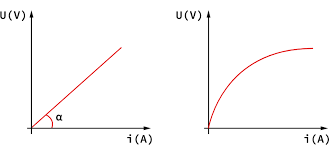
\includegraphics[width=0.7\textwidth]{resistor_ohmico.png}
    \caption{Gráficos da d.d.p. (U) pela corrente que passa num resistor ôhmico (à esquerda) e num resistor não-ôhmico (à direita)}
    \label{fig:resistores}
\end{figure}

\section{Potência dissipada por Efeito Joule}
Vimos na aula passada que, quando a corrente atravessa um material, uma parte da energia elétrica é dissipada em calor para o material, esquentando-o. Agora, nós vamos quantificar o quanto de potência dissipada um resistor ôhmico faz.

Lembremos que a potência é dada por $P=U\,i$ e que um resistor ôhmico respeita a Lei de Ohm: $U=R\,i$. Logo, substituindo a Lei de Ohm na equação da potência, temos que:
\begin{equation}\label{eq:power-1}
    P = (R\,i)\,i \implies \boxed{P= R\,i^2}
\end{equation}
Ou podemos reescrever da seguinte forma também:
\begin{equation}
    P = U\,\left(\frac{U}{R}\right) \implies \boxed{P = \frac{U^2}{R}}
\end{equation}

Ou seja, o valor da potência dependerá do valor da resistência desse resistor. \textbf{No caso de uma d.d.p. definida e constante, a potência aumenta conforme a resistência diminui e vice-versa. No caso de uma corrente definida e constante, a potência aumenta conforme a resistência é maior.}

Normalmente, é muito mais fácil de aplicar uma certa d.d.p. do que fornecer uma corrente constante, por isso, a relação da equação (\ref{eq:power-1}) tem uma importância maior. É possível determinar a resistência de um aparelho elétrico caso a sua potência e a sua tensão (d.d.p.) sejam fornecidas.

\section{2ª Lei de Ohm}
Georg Ohm, nos seus estudos, também percebeu que o valor da resistência de um resistor possuía certas dependências. A formulação que ele obteve foi a seguinte:
\begin{equation}
    R = \frac{\rho l}{A}
\end{equation}
\noindent em que $\rho$ é a resistividade do material que o resistor é feito, $l$ é o comprimento desse resistor e $A$ é a área de seção transversal do resistor.
\begin{figure}[H]
    \centering
    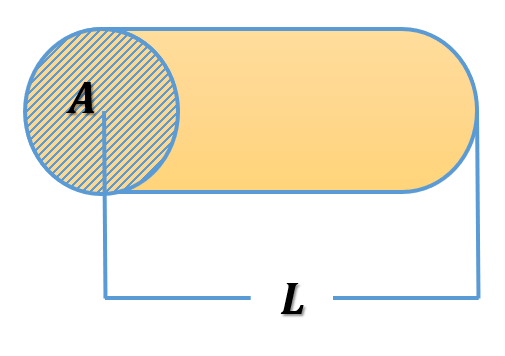
\includegraphics[width=0.35\textwidth]{condutor-segunda-lei-de-ohm-1.png}
    \caption{Diagrama das quantidades na 2ª Lei de Ohm}
    \label{fig:ohm_2}
\end{figure}

Uma questão importante é que resistores mais largos (maiores áreas de seção transversal) possuem resistência menor. Isso faz sentido, pois quanto mais espaço a corrente pode ocupar, mais facilmente ela pode ser conduzida, logo mais rápida ela pode andar no material. Outro ponto é que quanto mais longo for o resistor, a corrente tem um caminho difícil mais longo, portanto menos rápida ela vai andar.

Os valores das resistividades são valores tabelados e já estudados por cientistas e bem estabelecidos. A unidade da resistividade é $[\rho] =\Omega.m$

\section{Associação de Resistores}
\subsection{Associação em série}

\textbf{Quando os resistores estão em série, isso significa que o valor da corrente que passa no primeiro resistor é o mesmo que passa no segundo resistor.} 
\begin{figure}[H]
    \centering
    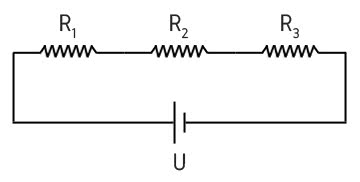
\includegraphics[width=0.4\textwidth]{resistores_em_serie.jpg}
    \caption{Diagrama de uma associação de resistores em série}
    \label{fig:serie}
\end{figure}

Logo, se eu aplicar a Lei de Ohm em cada resistor:
\begin{equation}
    \begin{split}
        U_1 &= R_1\,i\\
        U_2 &= R_2\,i
    \end{split}
\end{equation}

A diferença de potencial total ($U_{total}$) será a soma das diferenças de potencial ($U_1 + U_2$), então:
\begin{equation}
    \begin{split}
        U_{total} &= R_{eq}\,i\\
        U_1 + U_2 &= R_{eq}\,i\\
        R_1\,i + R_2\,i &= R_{eq}\,i\\
        (R_1+R_2)i &= R_{eq}\,i \implies \boxed{R_{eq} = R_1+R_2}
    \end{split}
\end{equation}

Esse resultado vale para mais de 2 resistores em série. Ou seja, \textbf{a resistência equivalente de um sistema de resistores em série é a soma das resistências}:
\begin{equation}
    R_{eq} = R_1+R_2+R_3 + \dots
\end{equation}

\subsection{Associação em paralelo}
\textbf{Quando os resistores estão em paralelo, os resistores estão sob uma mesma d.d.p. (U).} 
\begin{figure}[H]
    \centering
    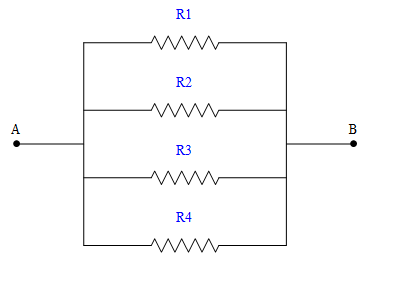
\includegraphics[width=0.4\textwidth]{resistencia_em_paralelo.png}
    \caption{Diagrama de uma associação de resistores em paralelo}
    \label{fig:paralelo}
\end{figure}

Então, pela Lei de Ohm:
\begin{equation}
    \begin{split}
        U &=R_1\,i_1\\
        U &=R_2\,i_2
    \end{split}
\end{equation}

Pela questão da continuidade da corrente elétrica, a corrente de entrada $i$ tem que ser a soma das corrente elétricas nos 2 resistores ($i_1 + i_2$), logo:
\begin{equation}
    U = R_{eq}\,i \implies i=\frac{U}{R_{eq}}
\end{equation}

Como $i=i_1+i_2$ (pela continuidade), então:
\begin{equation}
    \begin{split}
        i &= i_1+i_2 \\
        \frac{U}{R_{eq}} &= \frac{U}{R_1} + \frac{U}{R_2}\\
        U\left(\frac{1}{R_{eq}}\right) &= U\left(\frac{1}{R_1}+\frac{1}{R_2}\right) \implies \boxed{\frac{1}{R_{eq}} = \frac{1}{R_1}+\frac{1}{R_2}}
    \end{split}
\end{equation}
Esse resultado também vale para mais de 2 resistores em série. Em geral, a resistência equivalente é dada por meio dessa soma diferente, em que as resistências são o denominador da soma de frações. Enfim, o caso geral é dado por:
\begin{equation}
    \frac{1}{R_{eq}} = \frac{1}{R_1} + \frac{1}{R_2} + \frac{1}{R_3} + \dots
\end{equation}

\section{Ponte de Wheatstone}
O físico inglês Charles Wheatstone, durante os seus estudos de elétrica, descobriu uma relação entre resistores para uma formação de um circuito como o abaixo. No meio do circuito, colocamos um medidor chamado de \textbf{galvanômetro}.
\begin{figure}[H]
    \centering
    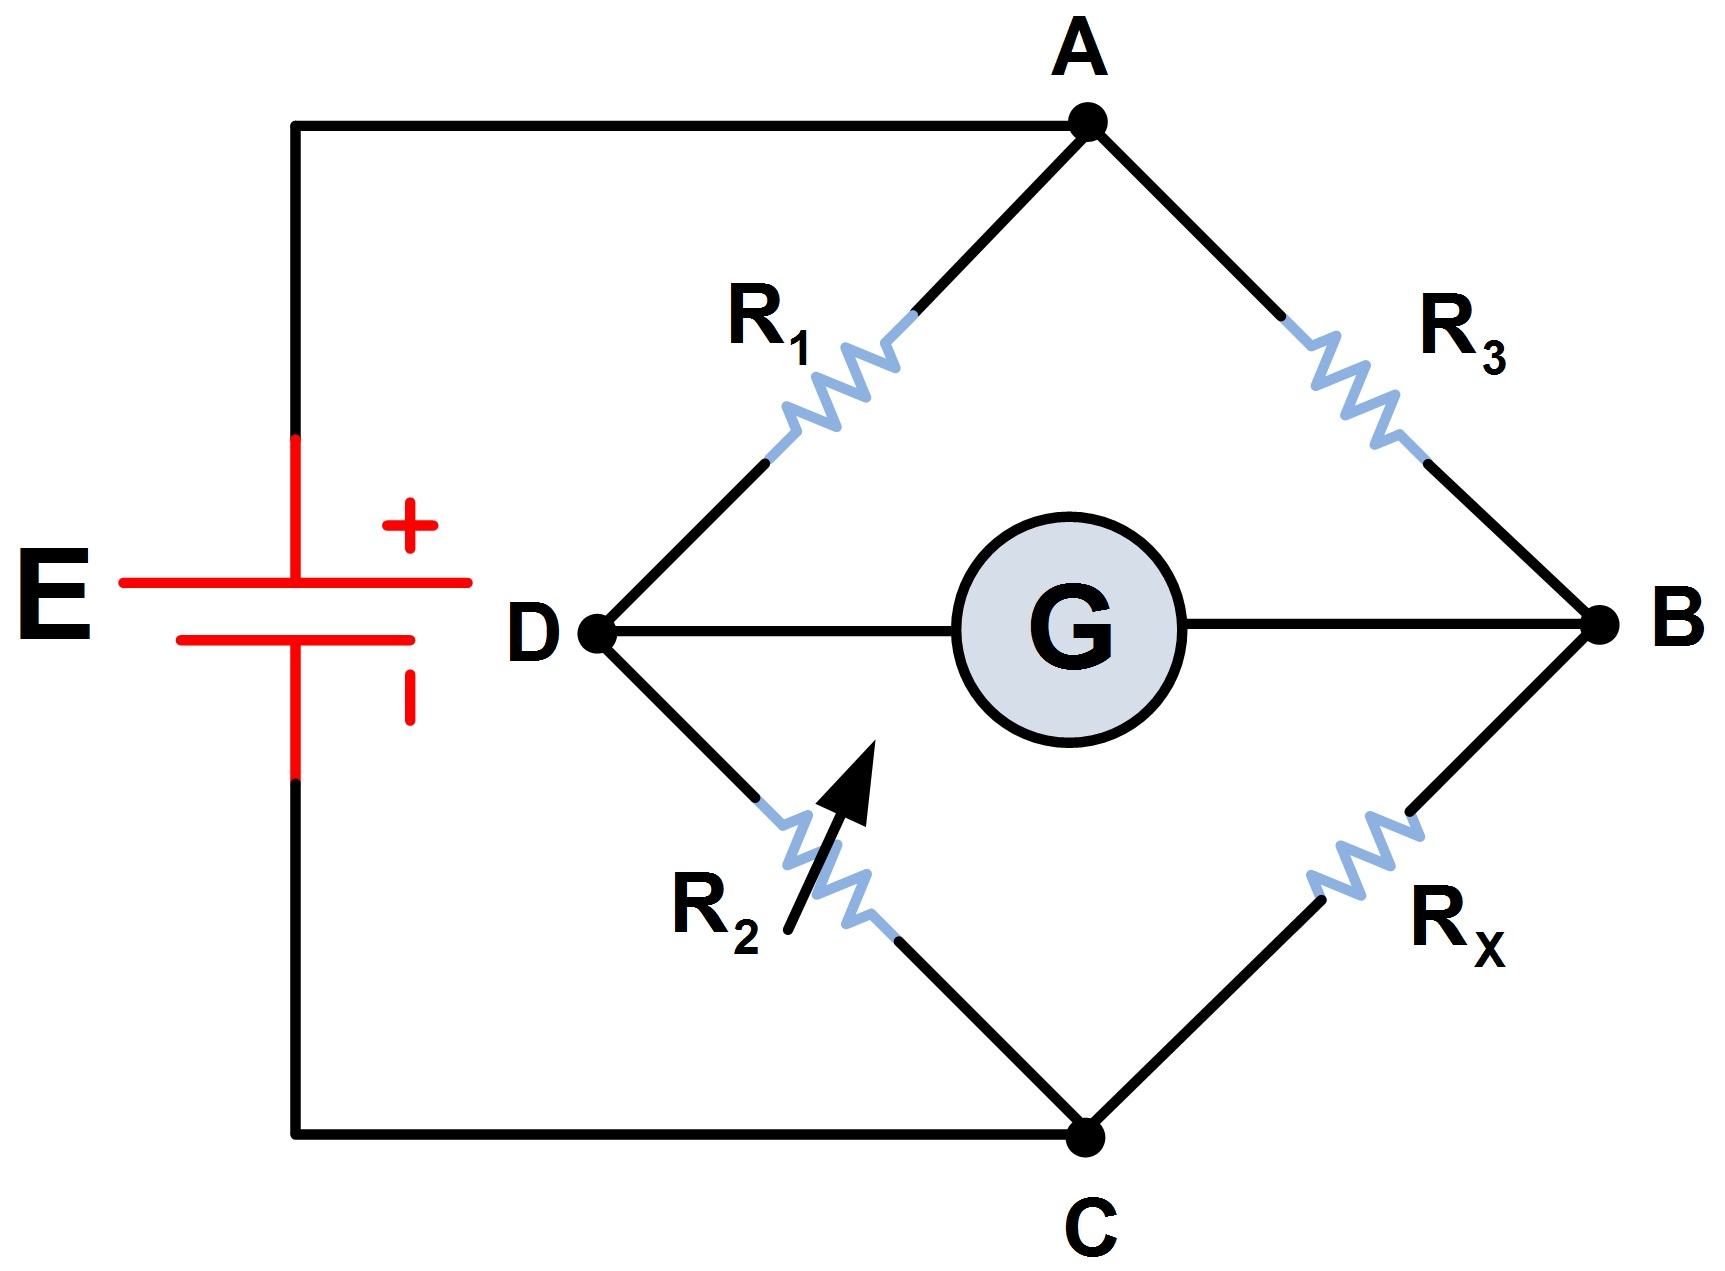
\includegraphics[width=0.6\textwidth]{wheat.jpg}
    \caption{Diagrama de uma Ponte de Wheatstone}
    \label{fig:wheatstone}
\end{figure}

\textbf{Quando o circuito está em equilíbrio, ou seja, quando o galvanômetro não mede nenhuma corrente passando por ele}, a relação entre os resistores é dada por:
\begin{equation}
    R_1\,R_4 = R_2\,R_3
\end{equation}
\end{document}
